% Sets the slides' look and contains some custom commands as well as colors
\input{../../Shared_Latex/custom_rochester.tex}
\input{../../Shared_Latex/author_and_date.tex}

% Quoting text
\usepackage{csquotes}

\title{Automata}

\usepackage{tikz}
\usetikzlibrary{automata, positioning}

\begin{document}

% Automata as graphs

\newcommand{\threeStateAutomaton}{
 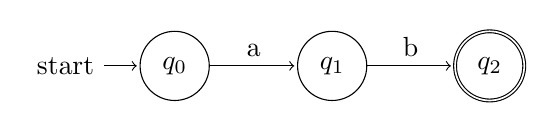
\begin{tikzpicture}[shorten >=1pt,node distance=2cm,on grid,auto]
   \node[state, initial] (q0) {$q_0$};
   \node[state] (q1) [right=of q0] {$q_1$};
   \node[state, accepting] (q2) [right=of q1] {$q_2$};
   \path[->]
    (q0) edge node {a} (q1)
    (q1) edge node {b} (q2);
 \end{tikzpicture}
}
\newcommand{\threeStateAutomatonInFirstState}{
 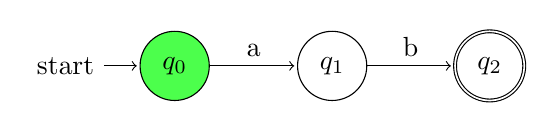
\begin{tikzpicture}[shorten >=1pt,node distance=2cm,on grid,auto]
   \node[state, initial, fill=green!70] (q0) {$q_0$};
   \node[state] (q1) [right=of q0] {$q_1$};
   \node[state, accepting] (q2) [right=of q1] {$q_2$};
   \path[->]
    (q0) edge node {a} (q1)
    (q1) edge node {b} (q2);
 \end{tikzpicture}
}
\newcommand{\threeStateAutomatonInSecondState}{
 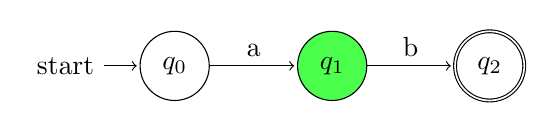
\begin{tikzpicture}[shorten >=1pt,node distance=2cm,on grid,auto]
   \node[state, initial] (q0) {$q_0$};
   \node[state, fill=green!70] (q1) [right=of q0] {$q_1$};
   \node[state, accepting] (q2) [right=of q1] {$q_2$};
   \path[->]
    (q0) edge node {a} (q1)
    (q1) edge node {b} (q2);
 \end{tikzpicture}
}
\newcommand{\threeStateAutomatonInThirdState}{
 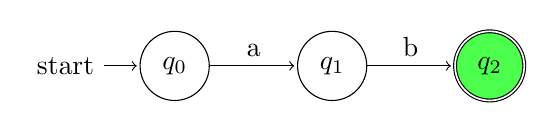
\begin{tikzpicture}[shorten >=1pt,node distance=2cm,on grid,auto]
   \node[state, initial] (q0) {$q_0$};
   \node[state] (q1) [right=of q0] {$q_1$};
   \node[state, accepting, fill=green!70] (q2) [right=of q1] {$q_2$};
   \path[->]
    (q0) edge node {a} (q1)
    (q1) edge node {b} (q2);
 \end{tikzpicture}
}

\maketitle
%%%%%%%%%%%%%%%%%%%%%%%%%%%%%%%%%%%%%%%%%%%%%%%%%%%%%
\frame{
  \frametitle{Today's Plan}
  \begin{itemize}
    \item What's an automaton (plural: \enquote{automata})?
    \item How do automata relate to grammars?
  \end{itemize}
}
%%%%%%%%%%%%%%%%%%%%%%%%%%%%%%%%%%%%%%%%%%%%%%%%%%%%%
\frame{
  \frametitle{Automata}
  \begin{itemize}
    \item An automaton consists of \textbf{states} % Maybe insert a circled q0
    \item An automaton can \textbf{transition} from state to state
    \item An automaton reads a string from left to right, one character at a time
    \item Each new character can put the automaton into a new state
    % TODO: Replace "final state" with "accepting state". Hopcroft and Ullman use this term on page 19 of "Introduction to Automata Theory, Languages, and Computation"
    \item If the automaton is in a \textbf{final}\footnote<5->{a better word for \enquote{final} is probably \enquote{accepting}} state after reading the last character, the string is valid
  \end{itemize}

  \threeStateAutomaton
}
%%%%%%%%%%%%%%%%%%%%%%%%%%%%%%%%%%%%%%%%%%%%%%%%%%%%%
\frame{
  \frametitle{Automata}

  \threeStateAutomaton

  \begin{itemize}
    \item This automaton has three states: $q_0, q_1, q_2$
    \item I has two transitions: \begin{enumerate}
        \item $\delta (q_0, a) = q_1$
        \item $\delta (q_1, b) = q_2$
    \end{enumerate}
  \item That means: \begin{enumerate}
      \item If the automaton is in state $\mathbf{q_0}$ and the current character of the input string is \enquote{\textbf{a}}, the automaton goes into state $\mathbf{q_1}$
      \item If the automaton is in state $\mathbf{q_1}$ and the current character of the input string is \enquote{\textbf{b}}, the automaton goes into state $\mathbf{q_2}$
  \end{enumerate}
\item $\delta$ (lowercase delta) is called the automaton's \textbf{transition function}
  \end{itemize}
}
%%%%%%%%%%%%%%%%%%%%%%%%%%%%%%%%%%%%%%%%%%%%%%%%%%%%%
\frame{
  \frametitle{Automata}
  \framesubtitle{Validating a String}

  \only<1>{\threeStateAutomaton}
  \only<2>{\threeStateAutomatonInFirstState}
  \only<3>{\threeStateAutomatonInSecondState}
  \only<4->{\threeStateAutomatonInThirdState}

  \begin{itemize}
    \item Does our automaton accept the string \enquote{ab}?
    \item The start state is $q_0$
    \item The first character in the string is \enquote{a} $\rightarrow$ The automaton transitions from $q_0$ to $q_1$
    \item The next character is \enquote{b} $\rightarrow$ The automaton transitions from $q_1$ to $q_2$
    \item We're done with the string: Is our automaton in a final state?
    \item Yes. Therefore, this automaton accepts the string \enquote{ab}
  \end{itemize}
}

%%%%%%%%%%%%%%%%%%%%%%%%%%%%%%%%%%%%%%%%%%%%%%%%%%%%%%
\frame{
  \frametitle{Automata and Grammars}
  \threeStateAutomaton
  \begin{itemize}
    \item This automaton corresponds to this grammar in extended Backus-Naur form (EBNF):
      \begin{itemize}[<.->]
        \item[] \texttt{a = "a";}
        \item[] \texttt{b = "b";}
        \item[] \texttt{sentence = a, b;}
      \end{itemize}
    \item The language specified by this automaton and grammar is $\{ab\}$
    \item If there's an automaton like this for a language, that language is called \textbf{regular}
  \end{itemize}
}
%%%%%%%%%%%%%%%%%%%%%%%%%%%%%%%%%%%%%%%%%%%%%%%%%%%%
\frame{
  \frametitle{Automata and Grammars}
  \begin{itemize}
    \item Let's consider this grammar:
      \begin{itemize}[<.->]
        \item[] \texttt{a = "a";}
        \item[] \texttt{b = "b";}
        \item[] \texttt{sentence = a, b, rest;}
        \item[] \texttt{rest = a, rest | b, rest | "";}
      \end{itemize}
    \item This grammar creates sentences like \enquote{ab}, \enquote{abaa}, \enquote{abba}
    \item They need to start with \enquote{ab}, the rest can be any letter from the alphabet
    \item What's the automaton for this grammar?
  \end{itemize}
}
%%%%%%%%%%%%%%%%%%%%%%%%%%%%%%%%%%%%%%%%%%%%%%%%%%%%
\frame{
  \frametitle{Automata and Grammars}
  \framesubtitle{Introducing Trap States}
 \begin{tikzpicture}[shorten >=1pt,node distance=3cm,on grid,auto]
   \node[state, initial] (q0) {$q_0$};
   \node[state] (q1) [right=of q0] {$q_1$};
   \node[state, accepting] (q2) [right=of q1] {$q_2$};
   \node[state] (q3) [below=of q1] {$q_3$};
   \path[->]
    (q0) edge node {a} (q1)
         edge node [swap] {b} (q3)
    (q1) edge node {b} (q2)
         edge node {a} (q3)
    (q2) edge [loop below] node {a|b} ()
    (q3) edge [loop below] node {a|b} ();
 \end{tikzpicture}

  \begin{itemize}
    \item $q_2$ is a final trap state: Once we're in it, the rest of the input string doesn't matter, the string will be accepted anyway
    \item $q_3$ is a non-final trap state: Once we're in it, the rest of the input string doesn't matter, the string will never be accepted
  \end{itemize}
}
%%%%%%%%%%%%%%%%%%%%%%%%%%%%%%%%%%%%%%%%%%%%%%%%%%%%
\frame{
  \frametitle{Run the Automaton}
  \begin{itemize}
    \item Note the state for each character and determine if the automaton is in a final or non-final state after the last character:
      \begin{enumerate}
        \item \enquote{ababb}
        \item \enquote{aab}
        \item \enquote{bbab}
        \item \enquote{aba}
      \end{enumerate}
  \end{itemize}
}
%%%%%%%%%%%%%%%%%%%%%%%%%%%%%%%%%%%%%%%%%%%%%%%%%%%%
\frame{
  \frametitle{Your Turn}
  \begin{enumerate}
    \item Write down the transitions of the previous automaton in $\delta$~notation
    \item Create an automaton from this grammar written in EBNF:
      \begin{itemize}[<.->]
        \item[] \texttt{rest = "a" | "b" | "";}
        \item[] \texttt{sentence = "X", rest;}
      \end{itemize}
    \item Create an automaton from this grammar written in EBNF:
      \begin{itemize}[<.->]
        \item[] \texttt{rest = "a" | "b" | "";}
        \item[] \texttt{sentence = "X", rest | "Y", rest;}
      \end{itemize}
    \item Write down the alphabets of the previous two grammars/automata
  \end{enumerate}
% \begin{itemize}[<.->]
%   \item[] $\delta (q_0, a) = q_1$
%   \item[] $\delta (q_0, b) = q_3$
%   \item[] $\delta (q_1, b) = q_2$
%   \item[] $\delta (q_1, a) = q_3$
%   \item[] $\delta (q_2, a) = q_2$
%   \item[] $\delta (q_2, b) = q_2$
%   \item[] $\delta (q_3, a) = q_3$
%   \item[] $\delta (q_3, b) = q_3$
% \end{itemize}
}
%%%%%%%%%%%%%%%%%%%%%%%%%%%%%%%%%%%%%%%%%%%%%%%%%%%%
\frame{
  \frametitle{Still Your Turn}
    Using the alphabet $\{0,1\}$, construct different automata that accept:
      \begin{enumerate}[<.->]
        \item strings of even length (think about whether the empty string has even length)
        \item strings with a length of at least five
        \item strings with an even number of 0s, for example \enquote{}, \enquote{1}, \enquote{010}, \enquote{00}
        \item strings with an even number of 0s and an odd number of 1s, for example \enquote{1}, \enquote{010}, \enquote{11001}
      \end{enumerate}
}
%%%%%%%%%%%%%%%%%%%%%%%%%%%%%%%%%%%%%%%%%%%%%%%%%%%%
\frame{
  \frametitle{Exercises}
  \framesubtitle{Creating Automata}
    Using the alphabet $\{a,b\}$, construct different automata that accept:
      \begin{enumerate}[<.->]
        \item strings containing exactly one a. For example: \enquote{a}, \enquote{abb}, \enquote{ba}.
        \item strings with at least two a's. For example \enquote{aa}, \enquote{abaa}, \enquote{baba}
        \item strings with no more than two a's
        \item strings with exactly two a's and at least one b. This automaton requires seven states. Hint: Name the states \enquote{oneA}, \enquote{twoAs}, \enquote{atLeastOneB}, etc.
        \item Write down the transitions of the first three automata in $\delta$~notation
      \end{enumerate}
}
%%%%%%%%%%%%%%%%%%%%%%%%%%%%%%%%%%%%%%%%%%%%%%%%%%%%
\frame{
  \frametitle{Exercises}
  \framesubtitle{Creating Automata from Grammars}
      Create an automaton for each of these three EBNF grammars. First, create a few example strings from the grammar.
      \begin{enumerate}[<.->]
       % A grammar generating strings with exactly one b
       \item \begin{itemize}[<.->]
               \item[] \texttt{sentence = as, "b", as;}
               \item[] \texttt{as = "" | "a", as;}
             \end{itemize}
       % A grammar where both the first and the last letter is an a
       \item \begin{itemize}[<.->]
          \item[] \texttt{sentence = "a" | "a", rest, "a";}
          \item[] \texttt{rest = "a", rest | "b", rest | "";}
        \end{itemize}
       % A grammar generating strings where both the first and the last letter are the same
       \item \begin{itemize}[<.->]
          \item[] \texttt{s = "a" | "b" | "a", r, "a" | "b", r, "b";}
          \item[] \texttt{r = "a", r | "b", r | "";}
        \end{itemize}
        % \item A grammar generating strings where strings have an odd number of b's.
      \end{enumerate}
}
%%%%%%%%%%%%%%%%%%%%%%%%%%%%%%%%%%%%%%%%%%%%%%%%%%%%
\frame{
  \frametitle{Exercises}
  \framesubtitle{Creating Automata \textit{and} Grammars}
    Using the alphabet $\{a,b\}$, construct different automata that accept the following strings and create grammars in EBNF that generate those strings:
      \begin{enumerate}[<.->]
        \item all strings with exactly two a's.
        % exactlyTwoAs = bs, "a", bs, "a", bs;
        % bs = "" | "b", bs;
        \item all strings with at least two a's.
        % atLeastTwoAs = rest, "a", rest, "a", rest;
        % rest = "" | "a", rest | "b", rest;
        \item all strings with no more than three a's.
        % noMoreThanThreeAs = bs, "a", bs | bs, "a", bs, "a", bs | bs, "a", bs, "a", bs, "a", bs;
        % bs = "" | "b", bs;
        \item all strings with at least three a's.
        \item all strings that start with a and end with b.
        % startWithAandEndWithB = "a", rest, "b"
        % rest = "a", rest | "b", rest | "";
        \item all strings with an even number of b's.
        % evenBs = "" | as | evenBs, "b", evenBs, "b", evenBs;
        % as = "" | "a", as;
      \end{enumerate}
}
%%%%%%%%%%%%%%%%%%%%%%%%%%%%%%%%%%%%%%%%%%%%%%%%%%%%

% "Introduction to Formal Languages" by Peter Linz:
% * Page 42 shows a minimal automaton with two nodes and an edge. Then proceeds to show a simple graph that determines whether a variable identifier is valid
% * Page 44 shows the state diagram of a bit adder and explains the correlation to physical computer design: "As this example indicates, the automaton serves as a bridge between the very high-level, functional description of a circuit and its logical implementation through transistors, gates, and flip-flops. The automaton clearly shows the decision logic, yet it is formal enough to lend itself to precise mathematical manipulation.  For this reason, digital design methods rely heavily on concepts from automata theory"

% Transducer example (page 46):
% Digital computers normally represent all information by bit strings, using some type of encoding. For example, character information can be encoded using the well-known ASCII system. For this exercise, consider the two alphabets {a, b, c, d} and {0, 1}, respectively, and an encoding from the first to the second, defined by a → 00, b → 01, c → 10, d → 11. Construct a transducer for decoding strings on {0, 1} into the original message. For example, the input 010011 should generate as output "bad".

% Let students draw a transition graph from the transition function δ (probably say that q0 is the initial state and list the final states). Make clear that the automaton has an alphabet and that the inputs to the transition function δ are symbols from that alphabet
% Page 50 offers an example for that and also discusses which strings the accepter accepts
% An accepter has an associated languages: the languages is the set of strings that the accepter (the automaton) accepts
% Maybe introduce set notation for formal languages `L = {aⁿb : n ≥ 0}`
% Exercise inspired by the one on page 52: `L = {aⁿbⁿ : n ≥ 0}`. Example strings: "", "ab", "aabb", "aaabbb". Is this possible for a DFA (deterministic finite automaton)?
% Page 55: an automaton rejecting input string if it contains "001", accepting all other strings
% From pages 56 and 83: A language is regular if there exists a finite accepter for it, therefore, every regular language can be discribed by a DFA or NFA. Chapter 3 dives into regular expressions
% I could present the definition of a regular language, as above, and have an exercise where students prove that a given language is regular by creating a DFA for it

%%%%%%%%%%%%%%%%%%%%%%%%%%%%%%%%%%%%%%%%%%%%%%%%%%%%%
\end{document}

